\section{简介}
\label{sec:I}
% 学习此类映射的可能性,为设计具有广泛适用性的深度学习框架开辟了一类新问题。传统神经网络是有限维欧氏空间(finite-dimensional Euclidean spaces)和 / 或有限基数集合(sets of finite cardinality)之间的映射,基于传统神经网络进行拓展需要新的思路。这涉及无穷维空间(infinite-dimensional spaces),例如输入和输出本身是定义在欧氏空间某一区域上的函数的情况。
学习函数空间(function spaces)之间的映射在科学与工程领域具有广泛应用。例如,在求解微分方程(differential equations)时,输入为系数函数(coefficient function),输出为解函数(solution function)。解决该问题的一种直接方法是将无穷维的输入和输出函数空间离散化(discretize)为有限维网格(finite-dimensional grids),并应用神经网络(neural networks)等标准学习模型。然而,这种方法会限制适用性,因为所学习的神经网络模型可能无法很好地泛化到训练数据离散化网格(discretization grid)之外的其他离散化(discretizations)情况。


为克服标准神经网络的这些局限性,我们构建(formulate)了一个用于学习算子的新型深度学习框架,称为 {\em 神经算子(neural operators)},它可直接在有界区域(bounded domains)上的函数空间之间进行映射。由于我们的神经算子是在函数空间上设计的,因此可以通过多种不同方法、在不同分辨率(resolution)水平下对其进行离散化,且无需重新训练。相比之下,标准神经网络架构严重依赖训练数据的离散化:对于不同离散化程度的数据,可能需要具有新参数的新架构才能达到相同的误差水平。我们还提出了 {\em 离散化不变(discretization-invariant)} 模型的概念,并证明我们的神经算子满足该性质,而标准神经网络则不满足。
% 此类神经算子模型一旦训练完成,便具有离散化不变性质:可在基础函数数据的不同离散化形式之间共享相同的模型参数。我们通过数值实验证明,对于数据的任意离散化形式,同一神经算子都能实现低误差,而标准前馈神经网络(feed-forward neural networks)和卷积神经网络(convolutional neural networks)则无法做到。在偏微分方程(partial differential equations, PDEs)场景下,我们通过数值实验证明,在固定分辨率下,所提出的方法与神经网络模型相比具有很强的竞争力,且比用于生成数据的偏微分方程求解器(PDE solvers)快几个数量级(orders of magnitude)。
% 最后,我们为所提出的神经算子建立了通用逼近定理(universal approximation theorem),证明它们能够以任意精度逼近线性和非线性算子(linear and non-linear operators)。
% 本文研究了偏微分方程模型衍生的各类解算子(solution operators)或流映射(flow maps);具体而言,我们研究了函数空间之间的映射,其中输入数据例如可以是初始条件(initial condition)、边界条件(boundary condition)或系数函数,而输出数据则是相应的解。我们针对以下算子开展了数值实验:一维泊松方程(one-dimensional Poisson equation)\citep {Evans}、一维时间相关伯格斯方程(time-dependent one-space-dimensional Burgers' Equation)\citep {Evans}、二维稳态达西流动(two-dimensional steady Darcy Flow)\citep {bear2012fundamentals} 以及二维时间相关不可压缩纳维 - 斯托克斯方程(time-dependent two-space dimensional incompressible Navier-Stokes Equation)\citep {constantin1988navier,lemarie2018navier,temam2001navier}。
%3.1 节(Subsection \ref {ssec:LR})介绍了本文工作的研究背景与相关背景信息。3.2 节(Subsection \ref {ssec:OC})详细阐述了我们的研究贡献,并概述了论文内容。本文引言部分在 3.3 节(Subsection \ref {ssec:related-work})结束,该节提供了文献综述(literature review)。

\vspace{2cm}

\subsection{我们的方法}
\label{ssec:OC}

\paragraph{离散化不变性模型 (Discretization-Invariant Models).}

我们提出了\textbf{离散化不变性}(discretization invariance)的精确定数学概念。我们要求任何具有固定参数数量的离散化不变性模型必须满足以下条件:
\begin{enumerate}[leftmargin=*]
    \item  能够作用于输入函数的任意离散化形式,即可以接受输入域($\mathbb{R}^{d_a}$中某有界子集)中的任意点集,
    \item 可以在输出域($\mathbb{R}^{d_u}$中)的任意点上进行求值,
    \item 当离散化被细化时,收敛到一个连续算子(continuum operator)。
\end{enumerate} 

\noindent 接受输入域和输出域中任意点的第一条和第二条要求是离散化不变性的自然需求,而第三条则确保了在离散化不断细化的极限情况下的模型一致性。例如,图神经网络(graph neural networks)~\citep{scarselli2008graph} 和变换器模型(transformer models)~\citep{vaswani2017attention} 具有分辨率不变性(resolution invariant),即它们可以在任何分辨率下接收输入,但当离散化被细化时,它们无法收敛到一个连续算子。此外,我们要求模型具有固定的参数数量;否则,随着离散化的细化,参数数量在极限情况下会变得无界,如图 \ref{fig:discretization-invariance} 所示。因此,离散化不变性的概念使我们能够定义在函数空间中具有一致性、并且可以应用于任何分辨率和任何网格上给定数据的神经算子模型。我们还证明了标准的神经网络模型不具有离散化不变性。

% \todo{zongyi: 能否添加一张关于机翼(air foil)网格细化的示意图?不规则的也可以。我们在这里是定义概念。}



\begin{figure}[h]
    \centering
    \includegraphics[width=0.8\textwidth]{Figs/discretization-invariance.png}
    \caption{Discretization Invariance}
    \label{fig:discretization-invariance}
    离散不变算子具有在网格细化时收敛的预测能力。
    An discretization-invariant operator has convergent predictions on a mesh refinement.
\end{figure}

\paragraph{神经算子 (Neural Operators).}

我们提出了神经算子(neural operators)的概念,用于学习在无限维函数空间(infinite-dimensional function spaces)之间进行映射的算子(operators)。我们提出的神经算子架构由多层组成,其中每一层本身是由非线性激活函数(non-linear activations)组合而成的算子。这确保了整体的端到端组合是一个算子,从而满足离散化不变性(discretization invariance)的性质。神经算子的关键设计选择在于其算子层(operator layers)。为了简化设计,我们将层限制为线性算子(linear operators)。由于这些层与非线性激活函数相结合,我们得到了具有强表达能力的神经算子模型,能够捕捉任何连续算子。后一性质被称为通用逼近性(universal approximation)。

上述神经算子的设计思路与标准神经网络的设计思路非常相似:在标准神经网络中,线性层(例如矩阵乘法、卷积)与非线性激活函数组合,并且我们可以在紧致域(compact domains)上实现对连续函数的通用逼近~\citep{hornik1989multilayer}。神经算子则是将神经网络中的有限维线性层替换为函数空间中的线性算子。

% 我们进一步证明,神经算子模型是作用于巴拿赫空间(Banach spaces)之间的算子的通用逼近器。众所周知,神经网络是函数的通用逼近器,意味着它们可以一致逼近任何定义在紧致域上的连续函数~\citep{hornik1989multilayer}。类似地,我们证明神经算子可以在巴拿赫空间的紧致集上一致逼近任何连续算子。
% 由于神经算子的普适性,研究其是否能够逼近任何算子是很有意义的。

%\begin{theorem}[算子的通用逼近性]
%\label{thm:univ_approx_informal}
%神经算子是算子的通用逼近器。在给定适当的输入和输出函数空间的情况下,神经算子可以在适当的拓扑结构下任意精确地逼近任何算子。
%\end{theorem}
% 该定理及相关的正式表述见第~\ref{sec:approximation_main}节;证明在附录中提供。%该定理表明,当在实践中使用神经算子来逼近一个算子时,从逼近理论的角度来看,无需担心模型类的容量问题。

%\paragraph{神经算子的性质 (Properties of Neural Operators).}

%\begin{theorem}[神经算子的离散化不变性]
%\label{thm:disc_inv_informal}
%神经算子满足上述离散化不变性的标准,一个固定的神经算子模型可以作用于用于表示输入函数的任何离散化形式。
%\end{theorem}
% 该定理的正式表述见第~\ref{sec:discritizational_invariance}节,相关讨论见第~\ref{sec:neuraloperators}节。
% 在本文中,我们证明了传统的神经网络不是离散化不变性模型,而经过轻微修改的变换器(transformers)是分辨率不变性(resolution invariant)模型。


我们正式地证明了具有固定参数数量的神经算子(neural operator)模型满足离散化不变性(discretization invariance)。我们进一步证明,神经算子模型是作用于巴拿赫空间(Banach spaces)之间的连续算子的通用逼近器(universal approximators),并且可以一致地逼近定义在巴拿赫空间紧致集上的任何连续算子。{\bf 神经算子是目前已知的唯一一类能同时保证离散化不变性和通用逼近性的模型。} 不同深度学习模型的比较见表~\ref{table:deeplearning_comparison}。以往的深度学习模型大多定义在固定的网格上,移除、添加或移动网格点通常会使这些模型不再适用。因此,它们不具备离散化不变性。

我们为神经算子中的线性算子层(linear operator layers)提出了几种设计选择,例如参数化的积分算子(parameterized integral operator),或如图~\ref{fig:NO_architecture}所示的在谱域(spectral domain)中的乘法操作。
具体而言,我们提出了四种实现神经算子框架的实用方法:基于图的算子(graph-based operators)、低秩算子(low-rank operators)、多极图基算子(multipole graph-based operators)和傅里叶算子(Fourier operators)。具体来说,对于基于图的算子,我们开发了一种Nystr\"om扩展方法,将神经算子的积分算子公式与任意网格上的图神经网络(GNNs)家族联系起来。对于傅里叶算子,我们考虑了神经算子的谱域公式,这在可以应用快速变换方法的场景下能够导出高效的算法。

我们对神经算子的四种实现形式进行了详尽的数值研究。数值结果表明,所提出的方法即使在标准神经网络设计所针对的分辨率下,也始终优于所有现有的深度学习方法。对于二维纳维-斯托克斯方程(Navier-Stokes equation),在学习整个流映射(flow map)时,该方法在雷诺数(Reynolds number)为20时达到小于1\%的误差,在雷诺数为200时达到8\%的误差。[雷诺数是流体力学中的一个无量纲数,用于预测流动模式的变化。]

所提出的傅里叶神经算子(FNO)的推理时间比用于生成纳维-斯托克斯问题数据的伪谱方法(pseudo-spectral method)快三个数量级——在$256 \times 256$的均匀空间网格上,FNO仅需$0.005$s,而伪谱方法需要$2.2$s \citep{chandler2013invariant}。% \todo{需要修改这个数据}
尽管在速度上具有巨大的优势,但该方法在用于下游应用(如求解贝叶斯逆问题)时,其精度并未下降。此外,我们证明了FNO在本文考虑的测试问题上对噪声具有鲁棒性。



\begin{figure}[t]
    \centering
    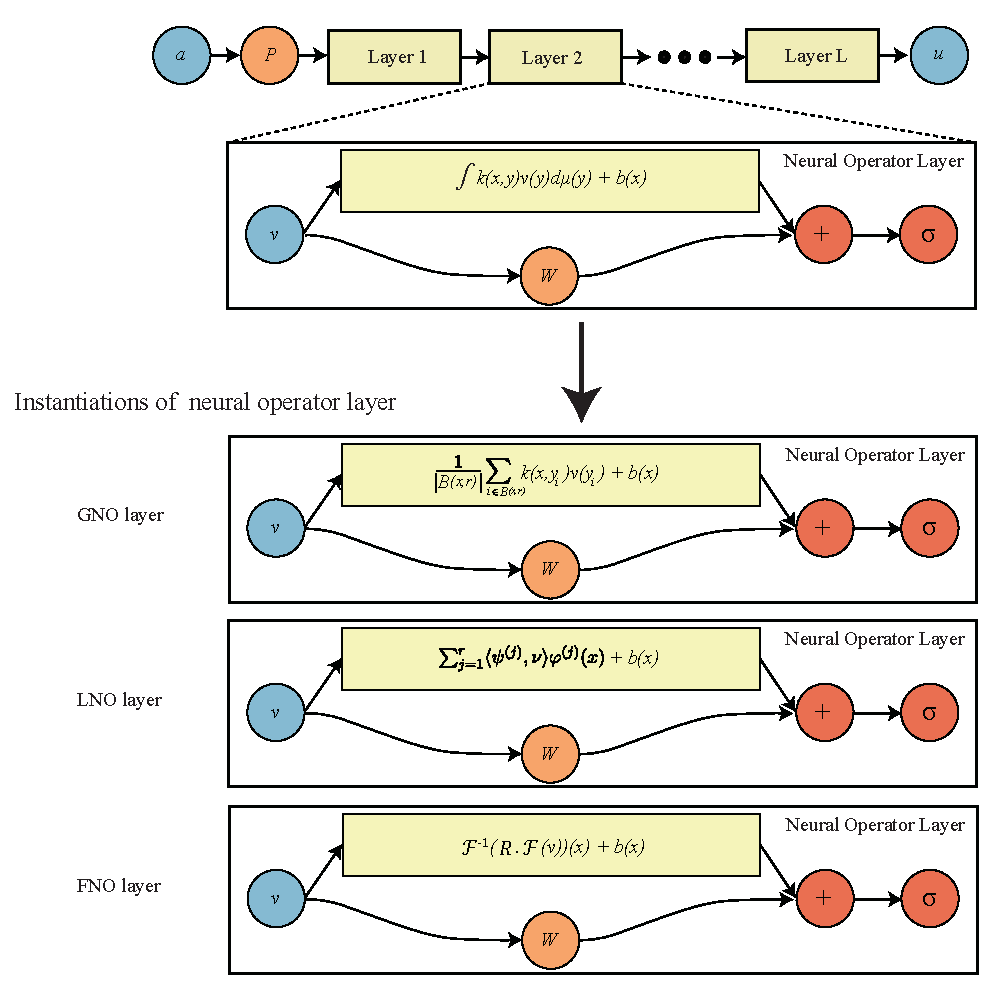
\includegraphics[width=0.8\textwidth]{Figs/NO-all-eq.pdf}
    \caption{Neural operator architecture schematic}
    \label{fig:NO_architecture} 
    \small{输入函数 $a$ 通过逐点提升算子 $P$,随后经过 $T$ 层积分算子和逐点非线性操作 $\sigma$。最后,逐点投影算子 $Q$ 输出函数 $u$。提供了神经算子层 GNO、LNO 和 FNO 的三种实例化方式。}
    \small{The input function $a$ is passed to a pointwise lifting operator $P$ that is followed by $T$ layers of integral operators and pointwise non-linearity operations $\sigma$. In the end, the pointwise projection operator $Q$ outputs the function $u$. Three instantiation of neural operator layers, GNO, LNO, and FNO are provided.}
\end{figure}



\begin{table}[h!]
\centering
\begin{tabular}{l|c|c|c|c}
% \diaghead{Scoreexp}{Property}{Model}&
\diagbox{Property\hspace{.5cm}}{\hspace{2em}\raisebox{-.3cm}{Model}}&
NNs& DeepONets & Interpolation & Neural Operators\\
\hline
Discretization Invariance & \xmark & \xmark & \cmark & \cmark \\
\hline
Is the output a function? & \xmark & \cmark & \cmark & \cmark \\
\hline
Can query the output at any point? & \xmark & \cmark & \cmark & \cmark \\
\hline
Can take the input at any point? & \nk{\xmark} & \xmark & \cmark & \cmark \\
\hline
Universal Approximation & \xmark & \cmark & \xmark & \cmark \\
\hline
\end{tabular}
\caption{深度学习模型的比较。第一行表示该模型是否具有离散化不变性。第二行和第三行表示输出和输入是否为函数。第四行表示该模型类是否为算子的通用逼近器。神经算子是离散化不变的深度学习方法,能够输出函数并逼近任意算子。}
\label{table:deeplearning_comparison}
\end{table}

\vspace{1cm}

\subsection{背景与相关工作}
\label{ssec:LR}
\paragraph{求解偏微分方程的数据驱动方法 (Data-driven approaches for solving PDEs).}
% ``微分方程[...]代表了人类为理解物质世界所创造的最强大的工具。'' \citet{strogatz2009loves}。
% 大量重要的工程和物理问题都由偏微分方程(PDEs)所支配。
在过去的几十年中,从微观尺度问题(例如,量子和分子动力学)到宏观尺度应用(例如,土木和海洋工程),许多科学领域的控制偏微分方程的建立 \citep{gurtin1982introduction} 和求解 \citep{johnson2012numerical} 方面都取得了显著进展。尽管偏微分方程在解决现实世界问题的应用上取得了成功,但仍然存在两个重大挑战:(1) 为复杂系统识别出其控制模型;(2) 高效地求解大规模非线性方程组。

识别并建立适用于特定问题的底层偏微分方程通常需要在相应领域内具备广泛的事先知识,然后结合普适的守恒定律来设计预测模型。例如,对固体结构的变形和失效进行建模,需要详细了解构成材料中的应力(stress)与应变(strain)之间的关系。对于活细胞等复杂系统,获得此类知识往往非常困难,为这些系统建立控制偏微分方程仍然难以实现,或者所提出的模型过于简单而缺乏信息量。从数据中获取此类知识的可能性将彻底改变这些领域。其次,求解复杂的非线性偏微分方程系统(例如湍流和塑性力学中出现的系统)在计算上要求很高,常常使得实际模拟变得不可行。同样,利用数据实例来设计快速近似求解器的可能性,对于加速众多问题具有巨大潜力。

\iffalse
\subsection{学习算子 (Learning the Operator)} 我们需要强调,学习算子 $\F$ 比求解单个方程的解 $u$ 是一项更具挑战性的任务。现有的大多数方法,从传统的有限元法(FEM)、有限差分法(FDM)到基于机器学习的物理信息神经网络(PINNs)\citep{raissi2019physics},它们的目标都是为单个方程找到解 $u$(即,针对单个 $a$ 进行一次求解)。另一方面,我们希望将 $\F$ 参数化为一个从 $a\in\A$ 到 $u\in\U$ 的映射。

与FEM和PINNs等偏微分方程求解器相比,神经算子通过学习解算子(solution operator),无需为每个方程单独求解。对于任何新的查询 $a$,它能立即输出评估结果。因此,它通常被用作一个快速求值器。例如,在逆问题中,当需要找到某些最优的材料结构 $a$ 时,神经算子可以快速评估输入 $a'$,并结合优化方法来寻找 $a' \to a$。
\fi


\paragraph{学习偏微分方程解算子 (Learning PDE Solution Operators).}
在偏微分方程(PDE)的应用中,控制微分方程根据定义是局部的(local),而解算子(solution operator)则表现出非局部(non-local)的特性。这种非局部效应可以通过空间域(spatial domain)中的积分算子(integral operators)显式地描述,或者通过谱域(spectral domain)中的乘法来实现;卷积(convolution)就是一个典型的例子。对于积分方程,Nystr\"om类型的图近似方法 \citep{belongie2002spectral} 为连接计算方法中出现的不同网格或数据结构并理解其连续极限(continuum limits)提供了一致的方法 \citep{von2008consistency,trillos2018variational,trillos2020error}。对于谱域计算,存在成熟的工具可用于逼近连续统(continuum)\citep{boyd2001chebyshev,trefethen2000spectral}。然而,这些逼近积分算子的方法并非数据驱动(data-driven)。神经网络为基于学习的积分算子逼近提供了一种自然的方法,因为它们可以融入非局部性。然而,标准的神经网络受限于训练数据的离散化方式,因此对积分算子的逼近效果较差。我们通过提出神经算子(neural operators)的框架来解决这一问题。

% 这是本研究背后的核心原则,旨在为偏微分方程解算子设计出与网格无关(mesh invariant)的神经网络逼近方法。

% 当监督学习被设计成能够模拟函数空间之间映射的方式时,它有潜力解决这些挑战 \citep{khoo2017solving,lu2019deeponet,Kovachki,nelsen2020random,li2020fourier,li2020multipole,li2020neural, patel2021physics, opschoor2020deep, schwab2019deep, o2020derivative, wu2020data}。

% 要使一个模型适用于函数空间,它必须能够在任何离散化形式上运行,这意味着它必须适用于任何网格或分辨率。所提出的离散化不变性定义是通用的,即离散化不变性模型适用于任何离散化、网格或分辨率。


\paragraph{现有深度学习模型的性质 (Properties of existing deep-learning models).} 

以往的深度学习模型大多定义在固定的网格上,移除、添加或移动网格点通常会使这些模型不再适用,如表~\ref{table:deeplearning_comparison}所示。因此,它们不具备离散化不变性(discretization invariant)。

一般来说,标准的神经网络(NN)(例如多层感知机(Multilayer Perceptron, MLP)、卷积神经网络(Convolutional Neural Networks, CNN)、ResNet和视觉变换器(Vision Transformers, ViT))将输入网格和输出网格视为有限维向量,由于其输入和输出必须位于具有固定位置的固定网格上,因此不是离散化不变的。
另一方面,物理信息神经网络(PINNs)\citep{raissi2019physics}中使用的逐点(pointwise)神经网络,将每个坐标作为输入,是离散化不变的,因为它可以并行地应用于每个位置。然而,PINNs仅代表单个实例的解函数,而没有学习从输入函数到输出解函数的映射。

一类特殊的神经网络是卷积神经网络(CNNs)。CNNs在网格细化时也不会收敛,因为它们各自的场会随着不同的输入网格而变化。另一方面,如果通过网格大小进行归一化,CNNs可以应用于具有不同分辨率的均匀网格,这会收敛到微分算子,其方式类似于有限差分法(finite difference method)。插值(Interpolation)是实现离散化不变性的一种基线方法。

虽然神经网络+插值(NNs+Interpolation)(或更一般地,任何有限维神经网络+插值)具有分辨率不变性(resolution invariant),并且其输出可以在任意点进行查询,但它们不是算子的通用逼近器(universal approximators of operators),因为其内部CNN模型的输入和输出维度被定义为一个有界数。

DeepONets \citep{lu2019deeponet} 是一类具有通用逼近性质的算子。DeepONets由一个分支网络(branch net)和一个主干网络(trunk net)组成。主干网络允许在任意点进行查询,但分支网络将输入限制在固定位置;然而,可以通过修改分支网络使该方法具有离散化不变性,例如使用 \citep{de2022cost} 中采用的基于主成分分析(PCA-based)的方法。

% 我们做出了以下贡献。
% \begin{enumerate}
% \item 我们提出了神经算子(neural operators),将神经网络从映射有限维欧几里得空间推广到映射无限维函数空间的深度学习模型。

% \item 通过构造,我们的架构共享相同的参数,无论在计算目的上输入和输出空间使用何种离散化方式。我们发展了离散化不变性的一般定义,并证明神经算子是离散化不变的深度学习模型。因此,神经算子能够实现零样本超分辨率(zero-shot super-resolution)。% 如图 \ref{fig:super2} 所示。

% \hold{\item 我们建立了逼近定理,保证神经算子具有足够的表达能力,可以任意好地逼近在函数空间之间映射的任何可测算子(measurable operator),这些函数空间选自一大类可能的巴拿赫空间(Banach spaces)。}



此外,我们证明了变换器(transformers)~\citep{vaswani2017attention} 是神经算子(neural operators)在具有结构化核(structured kernels)情况下的特例,这些核可以与变化的网格一起使用来表示输入函数。然而,常用的基于视觉的变换器扩展,例如ViT~\citep{dosovitskiy2020image},使用卷积在图像块(patches)上生成标记(tokens),因此,它们不是离散化不变性模型。
% 当神经算子被应用于并限制在固定网格上时,它们是神经算子的特例。

我们还证明,当所提出的神经算子仅应用于固定网格时,得到的架构与神经网络及其他算子学习框架相吻合。在这种简化情况下,输入函数在网格点上的点值是已知的。特别地,我们证明了最近提出的DeepONets~\citep{lu2019deeponet}(一种从有限维空间到无限维空间的映射)是神经算子架构的特例,即当神经算子仅限于固定输入网格时的情况。此外,通过引入对DeepONet架构的调整,我们提出了DeepONet-Operator模型,该模型完全融入了函数空间之间映射的完整算子学习框架。

% \item 数值实验展示了该方法学习椭圆型偏微分方程的格林函数、从多孔介质流体流动的PDE模型的系数到解的算子,以及从非线性对流-扩散PDE的初始条件到后续时刻解的算子的能力。

% \item 我们证明了神经算子方法在实验中与数值分析中的参数化逼近方法以及现有的深度学习方法具有竞争力。

% \end{enumerate}